\documentclass[a4paper, 11pt]{article}
\usepackage{enumitem}
\usepackage{geometry}
\usepackage{amsmath}
\geometry{letterpaper, margin=1in}
\usepackage{graphicx}
\graphicspath{ {images/} }





% change margins for solution
\newenvironment{solution}{%
	\begin{list}{}{%
			\setlength{\topsep}{0pt}%
			\setlength{\leftmargin}{0.5cm}%
			\setlength{\rightmargin}{0.5cm}%
			\setlength{\listparindent}{\parindent}%
			\setlength{\itemindent}{\parindent}%
			\setlength{\parsep}{\parskip}%
		}%
		\item[]}{\end{list}}


\begin{document}




\begin{enumerate}[leftmargin=0em, label=\textbf{\arabic*}.]
  \item The potential due to a ring of charge is given by:
    \[
      V(s,\phi,z) = \frac{1}{4\pi\epsilon_0}\frac{Q}{2\pi}\int_0^{2\pi}\frac{d\phi'}{\sqrt{s^2+R^2-2sR\cos(\phi-\phi')+z^2}}
    \]
    Expand this potential in a power series to fourth order, in the plane of the
    ring, for $s<R$. Warning: Make sure you keep \textbf{all} of the terms up to
    fourth order and none of the terms of higher order. This is tricky to do and
    is the most important lesson from this homework problem. \\
\end{enumerate}

\noindent\textbf{Solution:}
\begin{solution}
  \noindent To expand this potential in a power series, it would be nice to save
  some effort and use the series we have already memorized (Quiz 1). Recall,
  \begin{equation}
    (1+u)^p = 1+pu + \frac{p(p-1)}{2!}u^2+\frac{p(p-1)(p-2)}{3!}u^3+\frac{p(p-1)(p-2)(p-3)}{4!}u^4+ \cdots
  \end{equation}
  We are looking at the potential in the plane of the ring, so $z=0$. We can
  also rewrite the square root as a power.
  \begin{equation}
    V(s,\phi,z=0)=\frac{1}{4\pi\epsilon_0}\frac{Q}{2\pi}\int_0^{2\pi}\Big(s^2+R^2-2sR\cos(\phi-\phi')\Big)^{-1/2}d\phi'
  \end{equation}
  The integrand is almost the same as equation (1) but we need it to match
  exactly for the power series to be valid. \textbf{Remember:} equation (1) is
  valid only for $|u|<1$. We are interested in finding the potential where
  $s<R$, so we can \textit{pull out} $R^2$ from the expression. That is,
  \begin{align}
    \Big(s^2+R^2-2sR\cos(\phi-\phi')\Big)^{-1/2} &= \Big[R^2\Big(1+\frac{s^2}{R^2}-\frac{2s}{R}\cos(\phi-\phi')\Big)\Big]^{-1/2}\\
                                                 &= \frac{1}{R}\Big(1+\frac{s^2}{R^2}-\frac{2s}{R}\cos(\phi-\phi')\Big)^{-1/2} 
  \end{align}
  \begin{equation}
    u \equiv \frac{s^2}{R^2}-\frac{2s}{R}\cos(\phi-\phi'), \qquad p=-1/2
  \end{equation}
  where in the final line I have identified our $u$ and $p$ for the series
  expansion. \\
  
  \noindent Now, we need to expand the powers of $u$ in order to find all of the fourth
  order terms in $\frac{s}{R}$. Yes, this is a lot of algebra. 
  \begin{align}
    &(-1/2)u = \left( \frac{s}{R} \right)\cos(\phi-\phi')-\frac{1}{2}\left( \frac{s}{R} \right)^2\\
    &\frac{(-1/2)(-3/2)}{2}u^2 = \frac{5}{2}\left( \frac{s}{R} \right)^2\cos^2(\phi-\phi')-\frac{3}{2}\left( \frac{s}{R} \right)^3\cos(\phi-\phi')+\frac{3}{8}\left( \frac{s}{R} \right)^4 \\
    &\frac{(-1/2)(-3/2)(-5/2)}{6}u^3 = \frac{5}{2}\left( \frac{s}{R} \right)^3\cos^3(\phi-\phi')-\frac{15}{4}\left( \frac{s}{R} \right)^4\cos^2(\phi-\phi/) +...\\
    &\frac{(-1/2)(-3/2)(-5/2)(-7/2)}{24}u^4 = \frac{35}{8}\left( \frac{s}{R} \right)^4\cos^4(\phi-\phi')+...
  \end{align}
  Using this, the integral reduces to
  \begin{equation}
    \begin{split}
      V(s,\phi)\approx\frac{1}{4\pi\epsilon_0}\frac{Q}{2\pi}\frac{1}{R}\int_0^{2\pi}&\Bigg\{ 1+\cos(\phi-\phi')\left( \frac{s}{R} \right)\\
      &+ \left[ \frac{5}{2}\cos^2(\phi-\phi')-\frac{1}{2}  \right]\left( \frac{s}{R} \right)^2\\
      &+ \left[ \frac{5}{2}\cos^3(\phi-\phi')-\frac{3}{2}\cos(\phi-\phi')    \right]\left( \frac{s}{R} \right)^3\\
      &+ \left[ \frac{3}{8}-\frac{15}{4}\cos^2(\phi-\phi')+\frac{35}{8}\cos^4(\phi-\phi') \right]\left( \frac{s}{R} \right)^4  \Bigg\}d\phi'
    \end{split}
  \end{equation}

  \noindent The original equation for the potential can not be integrated analytically.
  Now that we have expanded the integrand, we have reduced the problem to a
  bunch of integrals of $\cos^n(\phi-\phi')$ which we can solve by 
  brute force. Before we proceed though, let's pause and think for a
  moment about the symmetries of the ring.\\
  

  \noindent The ring has cylindrical symmetry. The charge $Q$ is also evenly distributed
  along this ring. This means that the potential $V$ can not depend on $\phi$
  because if we were to close our eyes and rotate the ring, the new system would
  be indistinguishable from the original.
  \begin{figure}[!hbt]
    \centering
    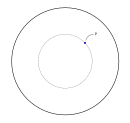
\includegraphics[width=0.7\columnwidth, angle=-90]{ring_symmetry}
    \caption{A point p within a ring of evenly distributed charge. All points
      along the dashed circle must have the same value of potential due to the
      symmetry of the charge distribution.}
  \end{figure}


  \noindent Thanks to the symmetry, we have the freedom to choose a value of $\phi$
  because the final solution \textit{can not} have $\phi$ dependence. For convenience,
  let's say $\phi=0$. Then our nasty integral can be further simplified to the
  following.  
 \begin{equation}
    \begin{split}
      V(s)\approx\frac{1}{4\pi\epsilon_0}\frac{Q}{2\pi}\frac{1}{R}\int_0^{2\pi}&\Bigg\{ 1+\cos(\phi')\left( \frac{s}{R} \right)\\
      &+ \left[ \frac{5}{2}\cos^2(\phi')-\frac{1}{2}  \right]\left( \frac{s}{R} \right)^2\\
      &+ \left[ \frac{5}{2}\cos^3(\phi')-\frac{3}{2}\cos(\phi')    \right]\left( \frac{s}{R} \right)^3\\
      &+ \left[ \frac{3}{8}-\frac{15}{4}\cos^2(\phi')+\frac{35}{8}\cos^4(\phi') \right]\left( \frac{s}{R} \right)^4  \Bigg\}d\phi'
    \end{split}
  \end{equation}

  \noindent In solving the above, the following integrals will be useful (look
  them up or try using the exponential form of cosine to solve).
  \begin{align}
    \int \cos(x) &= \sin(x)+C\\
    \int \cos^2(x) &= \int \frac{1}{2}(\cos(2x)+1)dx = \frac{1}{2}(x+\sin(x)\cos(x))+ C\\
    \int \cos^3(x) &= \frac{1}{12}(9\sin(x)+\sin(3x))+C\\
    \int \cos^4(x) &= \frac{1}{32}(12x+8\sin(2x)+\sin(4x)) + C
  \end{align}
  
  \begin{equation}
    \begin{split}
      V(s)\approx\frac{1}{4\pi\epsilon_0}\frac{Q}{2\pi}\frac{1}{R}\Bigg\{ 2\pi + &\left( \frac{s}{R} \right)\int_0^{2\pi}\cos(\phi')d\phi'\\
      &+ \left( \frac{s}{R} \right)^2\int_0^{2\pi}\left[ \frac{5}{2}\cos^2(\phi')-\frac{1}{2}  \right]d\phi'\\
      &+ \left( \frac{s}{R} \right)^3 \int_0^{2\pi}\left[ \frac{5}{2}\cos^3(\phi')-\frac{3}{2}\cos(\phi')    \right]d\phi'\\
      &+ \left( \frac{s}{R} \right)^4\int_0^{2\pi}\left[ \frac{3}{8}-\frac{15}{4}\cos^2(\phi')+\frac{35}{8}\cos^4(\phi') \right] d\phi' \Bigg\}
    \end{split}
  \end{equation}
  \begin{align}
    &= \frac{1}{4\pi\epsilon_0}\frac{Q}{2\pi}\frac{1}{R}\Bigg\{2\pi+ \frac{3\pi}{2}\left( \frac{s}{R} \right)^2 -3\pi\left( \frac{s}{R} \right)^4\Bigg\} \\
    &= \frac{Q}{4\pi\epsilon_0}\Bigg\{ \frac{1}{R}+\frac{3}{4} \frac{s^2}{R^3} -\frac{3}{2} \frac{s^4}{R^5}\Bigg\} \\
  \end{align}

  \textbf{NOTE:} our solution is an even function in $s$. Why is that? 

  
\end{solution}

\end{document}





















